\section{Query Optimizer Integration}
\label{discussion}

In the earlier sections, given a user query, the standard plan choice
of the Postgres optimizer was used even with the modified operator
implementations. That is, while the execution engine was PCM-conscious,
the presence of PCM was completely \emph{opaque} to the optimizer.
Given the read-write asymmetry of PCM in terms of both latency and wear
factor, it is possible that alternative plans, capable of providing better
performance profiles, may exist in the plan search space.  To discover
such plans, the database query optimizer needs to incorporate PCM
awareness in both the operator cost models and the plan enumeration
algorithms.

\begin{comment}
The above discussion is visually shown in Figure \ref{fig:layers}, wherein
the darkened squares indicate PCM awareness.
\begin{figure}[h]
	%\centering
	\subfloat[Database layers]{
	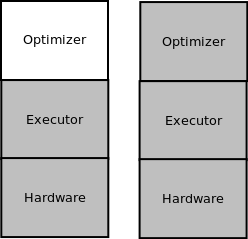
\includegraphics[width=4cm]{db_levels.png}
	}
   	\subfloat[Q13 alternate plan]{
   	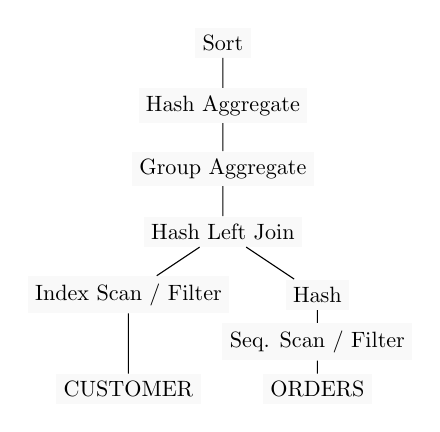
\begin{tikzpicture}[scale=.8, transform shape]

\tikzstyle{every node} = [rectangle, fill=gray!5]

\node (d) at (0,3) {Index Scan / Filter};
\node (c) at (0,1.5) {CUSTOMER};

\node (s) at (3,3) {Hash};
\node (p) at (3,2.25) {Seq. Scan / Filter};
\node (a) at (3,1.5) {ORDERS};

\node (e) at (1.5,4) {Hash Left Join};
\node (f) at (1.5,5)  {Group Aggregate};
\node (g) at (1.5,6)  {Hash Aggregate};
\node (h) at (1.5,7)  {Sort};


\draw[-] (c) -- (d);
\draw[-] (a) -- (p);
\draw[-] (d) -- (e);
\draw[-] (p) -- (s);
\draw[-] (s) -- (e);
\draw[-] (e) -- (f);

\draw[-] (f) -- (g);
\draw[-] (g) -- (h);

\end{tikzpicture}
   	}
  %\centering                                                                                             

\caption{Alternative Execution Plans for Query Q13}
	\label{fig:layers}
	
\end{figure}
\end{comment}

As a motivation for making the optimizer also PCM-aware, let
us revisit Query Q13, for which the default plan was shown in
Figure~\ref{fig:plan_trees}(a).  Now consider an alternative execution
plan wherein the merge left join between the \textit{customer} and
\textit{orders} tables is replaced by a hash left join.  The relative
performance of these two alternatives with regard to PCM Writes
and Cycles, are shown in Figures~\ref{fig:perf_comp}(a) and (b),
respectively. We observe here a \emph{huge difference} with regard to
both Writes and Cycles -- specifically, the alternative plan reduces
the writes by well over an order of magnitude!


\begin{figure}[htbp]
\centering
	
\subfloat[Performance of Alternative Plans]{
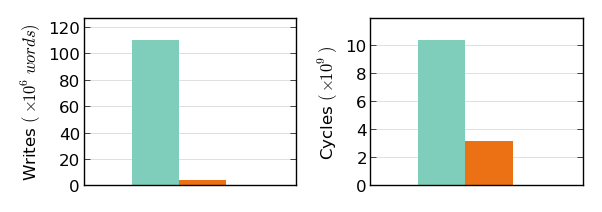
\includegraphics[height=29mm]{q13_alternate_plan.png}
}

\subfloat[Overall performance comparison]{
\begin{small}

  \begin{tabular}{p{1cm}p{1.6cm}p{1.6cm}p{1.6cm}}
  \toprule                                                                                                
  
  \textbf{Metric} & \textbf{Opt PCM-O Exec PCM-O } & \textbf{Opt PCM-O Exec PCM-C} & \textbf{Opt PCM-C Exec PCM-C}\\
  \midrule                                                                                                
  
  \textbf{Writes (words)} &  $233.6 \times 10^6$ & $110.6 \times 10^6$ & $4.66 \times 10^6$\\ 
  \textbf{Cycles} &  $13.1 \times 10^9$ & $10.4 \times 10^9$ & $3.2 \times 10^9$\\ 
  \bottomrule                                                                                             
  \end{tabular}                                                                                           
\end{small}                                                                                           
}
\caption{Performance comparison}
\label{fig:perf_comp}
\end{figure}

To put matters into perspective, Figure~\ref{fig:perf_comp}(b) summarizes
the relative performance benefits obtained as the database layers are
gradually made PCM-conscious (in the figure, the labels Opt and Exec refer to Optimizer and Executor, respectively, while PCM-O and PCM-C
refer to PCM-Oblivious and PCM-Conscious, respectively). The results
clearly indicate that future query optimizers for PCM-based architectures
need to incorporate these dual metrics of \emph{writes} and \emph{time}
in order to decide the most suitable plan for executing a given query.
